
% ==============================================================================
%
%                             Introduction
%
% ==============================================================================
\chapter{Introduction}
% Field/Context
Self driving cars are getting more popular and virtual reality video games
increasingly find their way into people's living rooms. One thing they share is
the need for a digital copy of the world. Self driving cars are trained in such
worlds to
accelerate the development of the algorithm and virtual reality games are
becoming more realistic. The Zurich based company Nomoko \footnote{
\url{https://www.nomoko.world/}} is developing a
technology that will enable the creation of digital copies of the world. They
built a giga pixel camera and a 3D pipeline to make this happen. This pipeline
consists among other things of high volume image processing. Modern computers
and graphical processing units (GPU) are fast in sequentially processing data
but are designed to serve many different tasks and not a specific one. A
dedicated hardware approach designed for a specific image processing task would
expedite the 3D pipeline of creating digital copies of the world.
\\

% Project goal/aims
The goal of this project is to implement such an image processing task on a
Field
Programmable Gate Array (FPGA). FPGAs
consist of thousands of logical elements that can be configured and connected
together to form a complex logical operation. Together with on chip
memory they offer high throughput by processing the data parallel in contrast to
sequential. The data is transfered to the FPGA over an Ethernet LAN connection
for
fast transfer rates. To accelerate the computing even further, the system needs
to be scalable to multiple FPGA boards to distribute the workload.
\\

% Primary objectives
Thus, two primary objectives can be defined:
\begin{enumerate}
    \item The image needs to be transfered from a computer to the FPGA board and
    back
    \item The image data on the FPGA must be processed using a common
    image processing task
\end{enumerate}
\begin{figure}[t!]
    \centering
    % \tikzsetnextfilename{system-overview}
\begin{tikzpicture}[
    rounded corners=0mm,
]
    %coordinates
    \coordinate (corig)      at (0,0);
    \coordinate (cmonitor)   at (0,0);
    \coordinate (ccom)       at (5,0);
    \coordinate (cip)        at (10,0);


    %nodes

    \begin{pgfonlayer}{main}
        \node[draw, fill=white, minimum width=3.2cm, minimum height=1.8cm, anchor=west, align=center, rounded corners=1mm] (mon) at (cmonitor) {};

        \node[draw, fill=white, minimum width=2.1cm, minimum height=0.4cm, anchor=west, align=center, rounded corners=2mm, below=0.2cm of mon] (stand) {};
        \node[draw, fill=white, minimum width=0.2cm, minimum height=0.1cm, anchor=south, align=center] (stange) at ($(stand.90) + (0,-0.04)$) {};



        \node[draw, fill=white, minimum width=3cm, minimum height=1cm, anchor=west, text width=2.8cm, align=center, right = 2cm of mon] (com) at (ccom) {Communication};

        \node[draw, fill=white, minimum width=3cm, minimum height=1cm, anchor=west, text width=2.8cm, align=center, right = 1cm of com] (ip) {Image\\Processing};
        

        \node[inner sep=0pt, anchor=west] (whitehead) at ($(cmonitor) + (0.1,0)$)
            {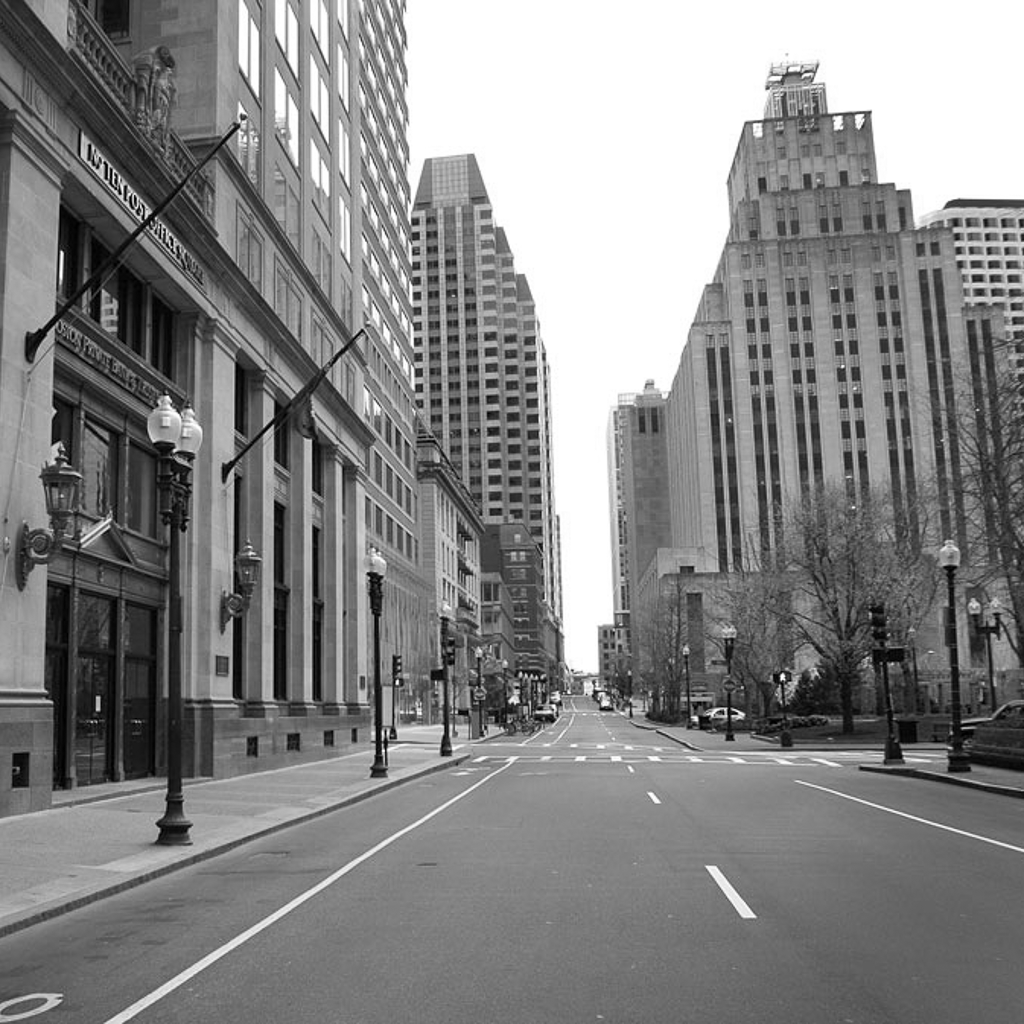
\includegraphics[width=1.4cm]{images/introduction/street1024.png}};
        \node[inner sep=0pt, anchor=west] (whitehead) at ($(cmonitor) + (1.7,0)$)
            {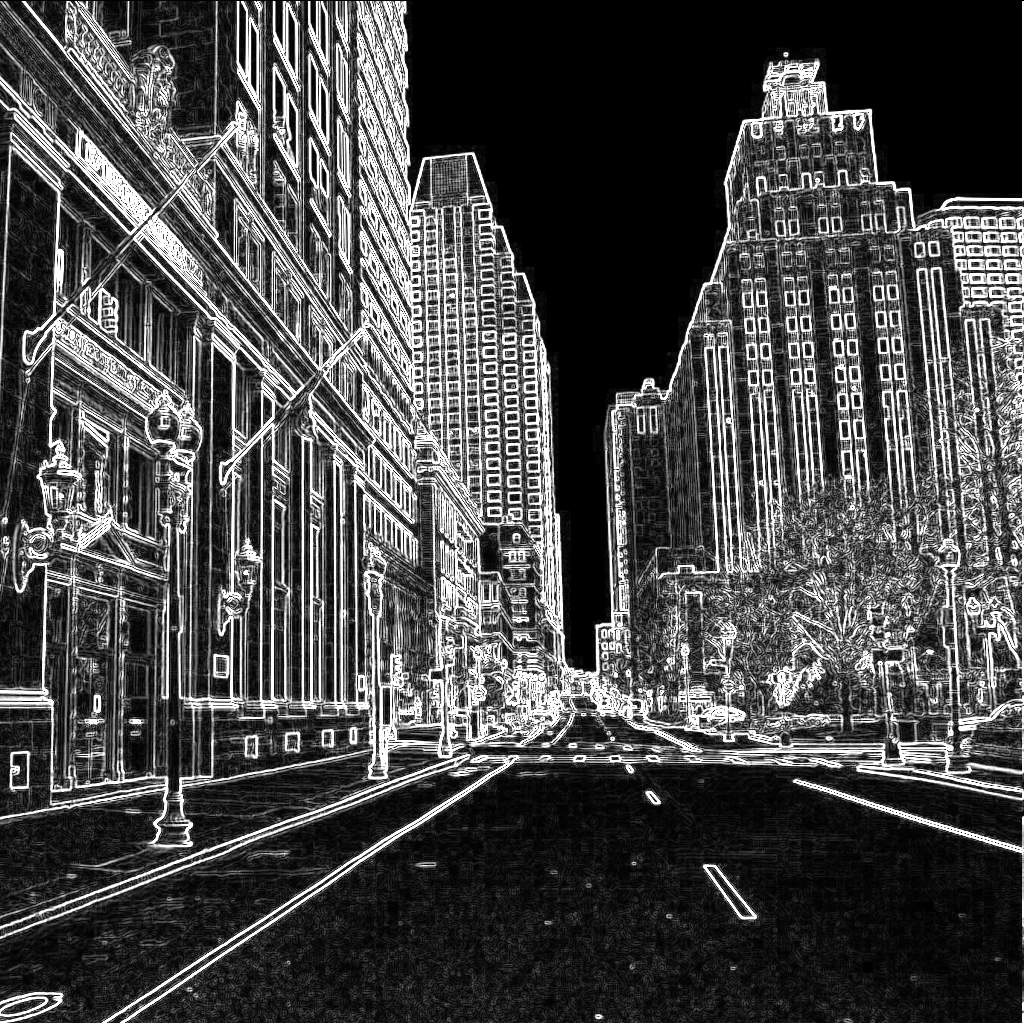
\includegraphics[width=1.4cm]{images/introduction/c_street1024.png}};

        \node[] (eth) at ($(cmonitor) + (4.5, 1.0)$) {LAN};
        
        \draw[line width = 0.5mm] ($(eth) + (0,-1.0)$) ellipse (0.2cm and 0.5cm);
    \end{pgfonlayer}

    % FPGA box
    \begin{pgfonlayer}{main}
        \node[above = 0.2cm of com, xshift=-1.5cm] (fpga) { FPGA };
    \end{pgfonlayer}
    \begin{pgfonlayer}{foreground}
        \node (f_fpga) [draw=black, fill=gray!20, inner sep=20, fit={(com) (ip) }] {};
    \end{pgfonlayer} 

    
    \path[draw,-{Latex[length=2.5mm]}] ($(mon.0) + (0,0.2)$) -- ($(com.180) + (0,0.2)$) node[near end, above] () {1.} ;
    \path[draw,{Latex[length=2.5mm]}-] ($(mon.0) + (0,-0.2)$) -- ($(com.180) + (0,-0.2)$) node[near end, below] () {4.} ;

    \path[draw,-{Latex[length=2.5mm]}] ($(com.0) + (0,0.2)$) -- ($(ip.180) + (0,0.2)$) node[midway, above] () {2.} ;
    \path[draw,{Latex[length=2.5mm]}-] ($(com.0) + (0,-0.2)$) -- ($(ip.180) + (0,-0.2)$) node[midway, below] () {3.} ;

\end{tikzpicture}
    \caption{Data Flow}
    \label{fig:datafl}
\end{figure}

% What is used to realize...
To realize an Ethernet communication multiple protocols and standards must be
implemented. Ready to use solutions are available. These are compared and
selected. To keep it simple, User Datagram Protocol (UDP) is chosen for
transport layer. Due to UDP's lack of reliable data transfer a session protocol
is defined on top of UDP. This UDP file transfer protocol is implemented using
hardware description language (HDL).

When working with mathematically more complex problems like image processing,
writing the code in hardware description language is complex and
incomprehensible. Therefore a high level synthesis (HLS) approach is put to use.
The algorithm is described and thoroughly tested in C/C++ and then synthesized to
HDL by the Xilinx Vivado HLS toolchain. A Sobel filter operation is chosen as
image processing task to detect edges in the source image. This operation is
rather simple but serves the purpose of this project and can be used for
improved edge detection algorithms.

An Artix7 Evaluation Kit by Xilinx serves as a development and testing platform.
It is equipped with gigabit Ethernet LAN and an FPGA with sufficient logic
elements and memory for both the communication and image processing task.
\\

% What is the result of the project
The result is an image processing core that runs a Sobel filter operation on an
input
image to detect edges. It processes one eight-bit pixel per clock cycle at
100MHz
resulting in a 100 megapixels per second throughput. The
data is read from FPGA block memory and stored there as well. An Ethernet
communication stack written in VHDL handles layers two through five of the OSI
model and transfers data at 8.9 MB/s to a computer using a custom file
transfer protocol.
\\

% How the document is built up
This report is split into five main parts: Theoretical background, mission,
image processing, communication and verification. 
The theoretical background starting
on page \pageref{chapt:theoreticalback} explains the basics of image
processing, FPGA and Ethernet communication. Starting on page 
\pageref{chapt:mission} the chapter mission will cover the starting point and
presents the concept. Chapters \ref{chapt:image_processing} and \ref{chapt:dataflow} cover the actual implementation process of the image processing and communication parts
before verifying these components in chapter \ref{chapt:ver_bench} starting
on page \pageref{chapt:ver_bench}.

